\chapter{Phase 1 FPix upgrade modules}

In chapter \ref{ch:cms}, a description of the CMS pixel detector used during the collection of the data sets used in this analysis, was presented. During the extended year-end technical stop (EYETS) 2017, the complete CMS pixel detector was replaced in order to support the full performance of the CMS experiment under the higher radiation conditions produced by the increasing instantaneous luminosities delivered  by the LHC accelerator. It also was designed to address and mitigate the identified weaknesses in the previous system.

In this chapter, a description of the upgraded detector will be presented, making emphasis on the contributions made by the University of Nebraska - Lincoln (UNL) HEP group, which consisted of the assembly of about 600 of the modules that make up the phase 1 upgraded forward pixel detector (FPix).     

\subsection{The phase 1 FPix upgrade }

The previous pixel detector was designed to record efficiently and with high precision the first three space-points near the interaction region, in the range of $|\eta|<2.5$,  at a instantaneous luminosity of $1\times10^{34}$ cm$^{-2}$s$^{-1}$ and a bunch crossing each 25 ns. An average pileup of about 25 simultaneous overlapping events is expected. The incresaing luminosity would affects the performance of the detector reducing track reconstruction efficiency, and increasing the data loses caused by the degradation of the readout system; furthermore, if the LHC runs with 50 ns bunch spacing at twice the luminosity, then the data losses would increase almost exponentially, to losses of 50\% for the innermost layer. An ilustration of the foreseen reduced performance in tracking efficiency and data loss is shown in Figure \ref{fig:reduced_performance} in the case of simulated \ttbar events at instantaneous luminosities up to $2\times10^{34}$ cm$^{-2}$s$^{-1}$ with 25 ns and 50 ns bunch spacing.\cite{tdr}. The increasing fake rate is also showed. In conclusion, the prevoius pixel detector was not able to perform efficiently under the new luminosoty, pileup, radiation, and running conditionms.  

\begin{figure}[!h]
\centering
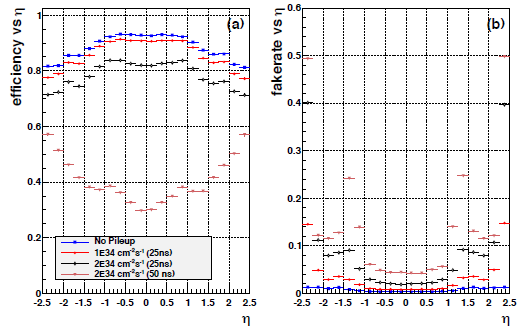
\includegraphics[width=0.9\textwidth]{pixel/reducedperformance2}
%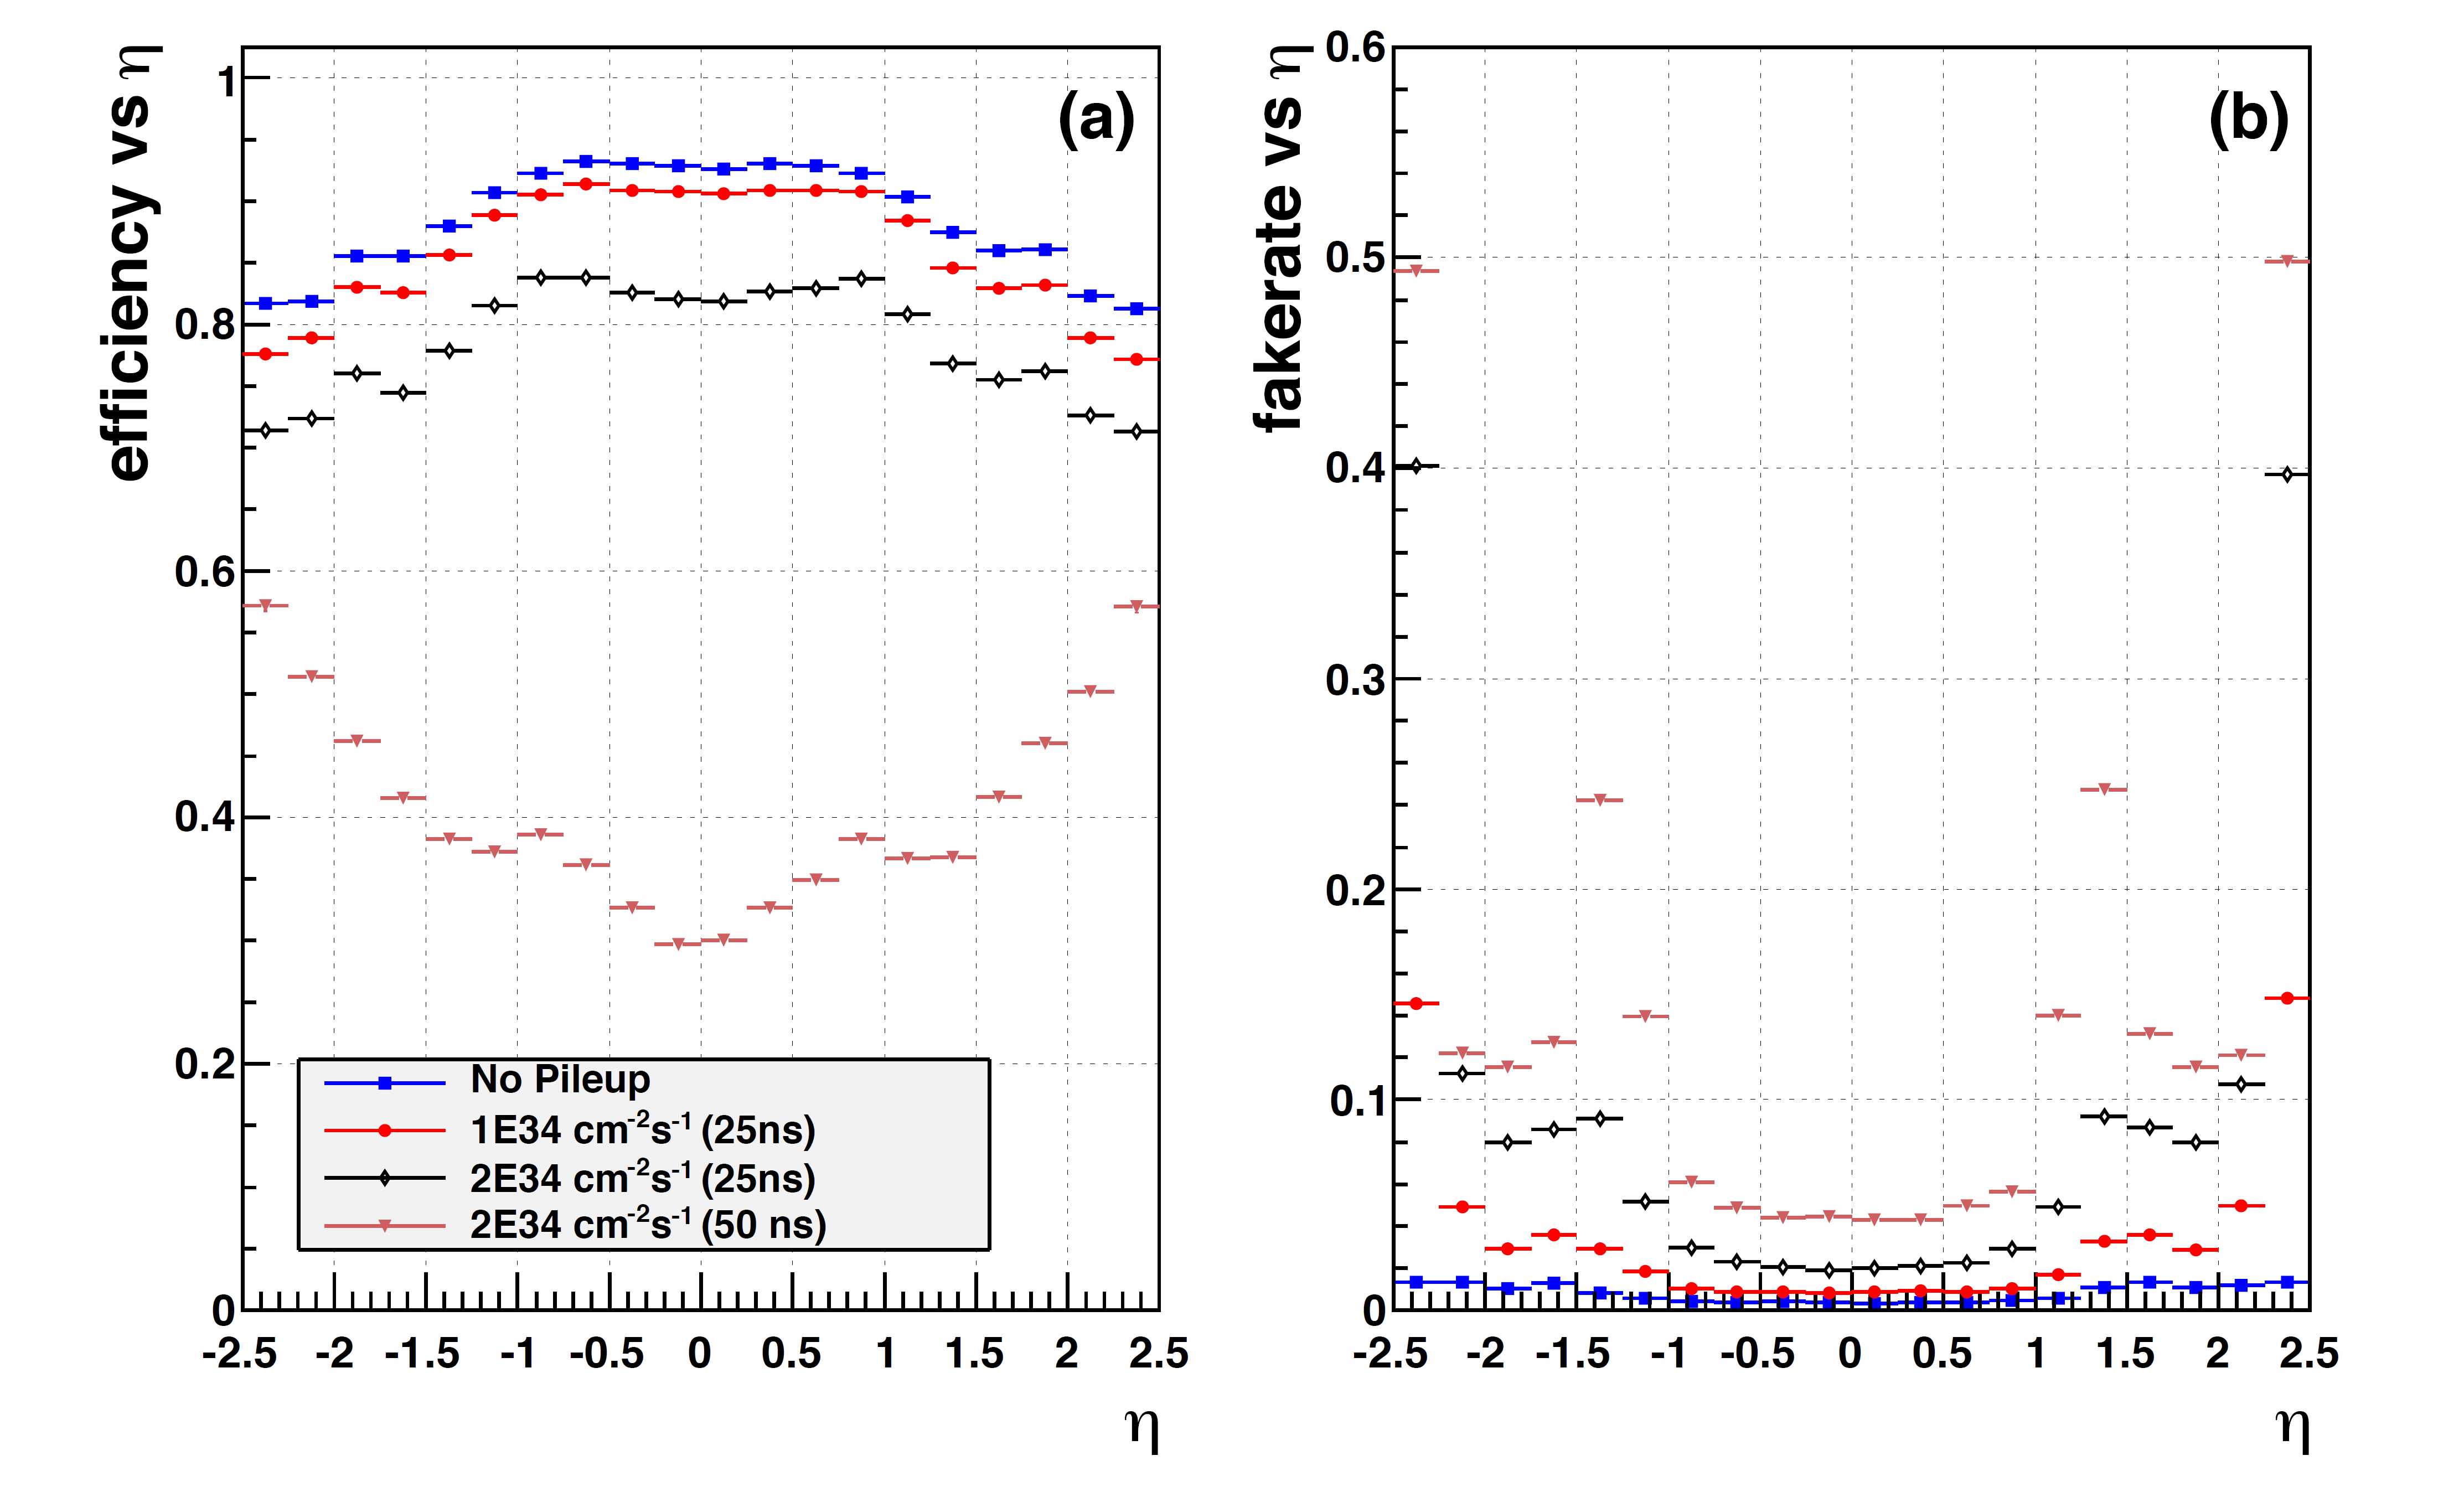
\includegraphics[width=0.9\textwidth]{pixel/reducedperformance}
\caption {Expected performance of the previous pixel detector in simulated \ttbar events: a) efficiency; b) fake rate. Conventions are the same for both plots.}\label{tdr}
\label{fig:reduced_performance}
\end{figure}

The present system is composed of four-layers/three-disks, low mass silicon pixel detectors providing a high performance tracking in the high luminosity environment.





%% \begin{figure}[!h]
%% \centering
%% 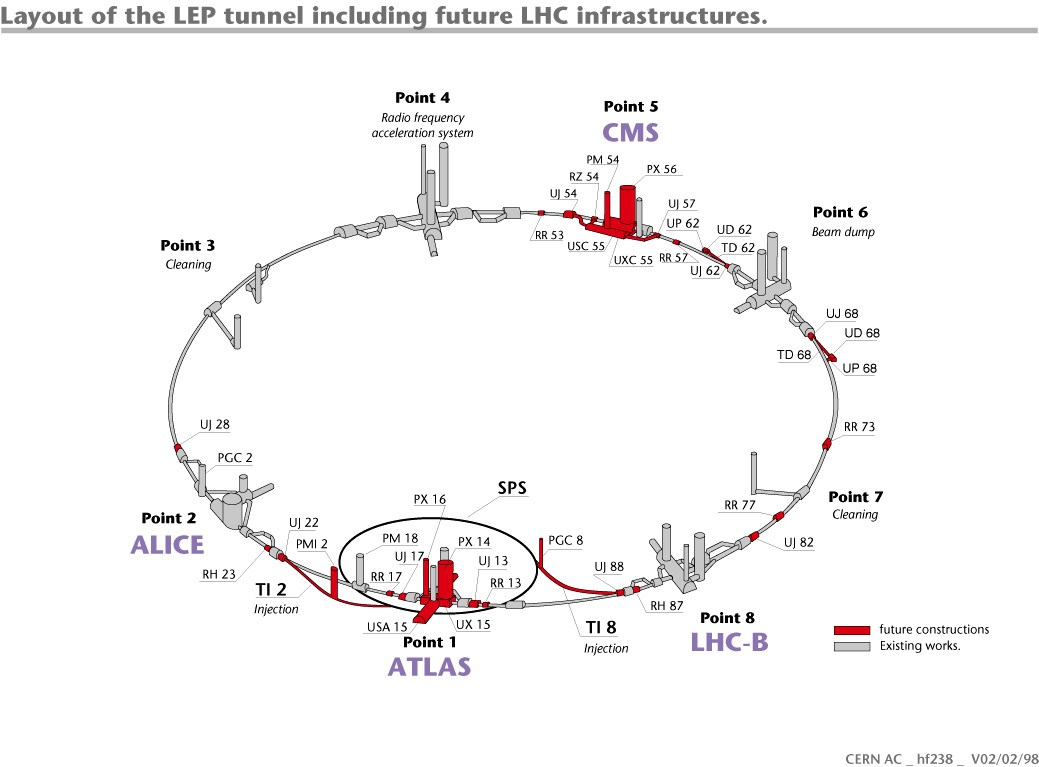
\includegraphics[scale=0.25]{lep}
%% \caption {ref.  }\label{lep}
%% \end{figure}

\subsection{FPix module production line}


%% \begin{figure}[!h]
%%   \centering
%%   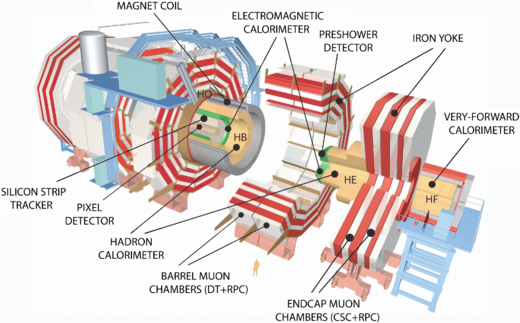
\includegraphics[scale=0.25]{cms}
%%   \caption {ref:  }\label{cms}
%% \end{figure}



\subsection{The Gluing stage}


%% \begin{figure}[!h]
%%   \centering
%%   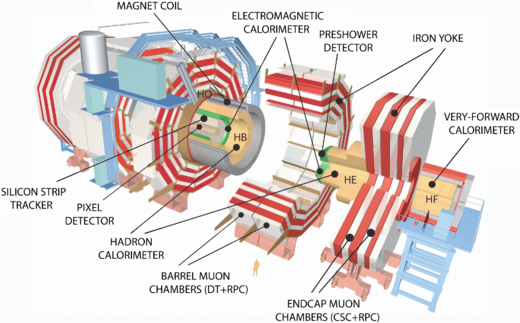
\includegraphics[scale=0.25]{cms}
%%   \caption {ref:  }\label{cms}
%% \end{figure}

\subsection{The Encapsulation stage}

%% \begin{figure}[!h]
%%   \centering
%%   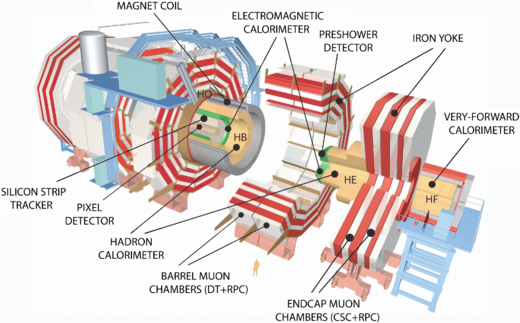
\includegraphics[scale=0.25]{cms}
%%   \caption {ref:  }\label{cms}
%% \end{figure}

\subsection{The FPix module production yields}

%% \begin{figure}[!h]
%%   \centering
%%   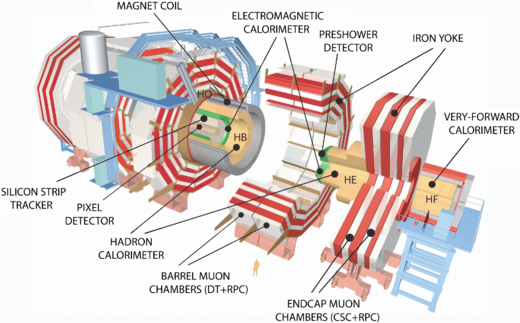
\includegraphics[scale=0.25]{cms}
%%   \caption {ref:  }\label{cms}
%% \end{figure}
